\documentclass[10pt]{article}
\usepackage[margin=0.8in]{geometry}
\usepackage{graphicx,booktabs,amsmath,hyperref,caption,array}
\usepackage{microtype}
\setlength{\textfloatsep}{8pt plus 2pt minus 2pt}\setlength{\floatsep}{6pt plus 2pt minus 2pt}\setlength{\abovecaptionskip}{3pt}\renewcommand{\topfraction}{0.9}\renewcommand{\textfraction}{0.1}\renewcommand{\floatpagefraction}{0.8}
\captionsetup{font=small,labelfont=bf}
\setlength{\parskip}{0.25em}
\setlength{\parindent}{0pt}
\newcommand{\ms}{\,ms}

\title{\vspace{-1em}CPU/GPU/NPU-Aware RAG Pipeline on an Intel Core Ultra:\\Phase 1 Measurement and Profiling Report}
\author{Ting-Yu Yu, Cheng-Yang Wu, Jonas Tsai, Vincent Chen}
\date{CSE 291A, Fall 2026 \;--\; Phase 1 (due Nov 4)}

\begin{document}
\maketitle
\vspace{-2em}

\section{Goal and summary}
Our project asks where each stage of an edge RAG pipeline should run on a machine whose CPU, integrated GPU (iGPU) and NPU share one DRAM. The pipeline is: query $\rightarrow$ \textbf{S1} embedding (bge-small-en-v1.5) $\rightarrow$ vector search $\rightarrow$ \textbf{S2} rerank (bge-reranker-base) $\rightarrow$ \textbf{S3} generation (Qwen2.5-1.5B-Instruct, INT4). Each model is loaded once on one device; there is no per-request routing. Phase 1 only measures. It answers three questions: can every stage run on every device, how fast and at what cost, and why do devices differ.

\textbf{Main findings.}
\begin{itemize}\setlength\itemsep{0pt}
\item All 9 stage$\times$device combinations run on the requested device, with no runtime fallback.
\item The iGPU is the fastest device for S2 and S3 at every size we measured. The NPU is competitive only for small encoder inputs (S1 batch 1; S2 with 10 candidates) and degrades sharply for larger shapes. The CPU is 15--20$\times$ slower for S2 and for S3 prefill.
\item End to end, all stages on the iGPU is best for latency, throughput up to $\sim$2.4 queries/s, and answer quality. Moving S2 to the NPU adds 110--140\,ms per query when S3 is on the iGPU or CPU (nothing when S3 is also on the NPU), lowers recall@3 from 0.87 to 0.82--0.83, and gives at most a few percent more capacity.
\item Placing S1 on any device changes end-to-end latency by about 20\,ms or less; S1 is irrelevant to the decision.
\item Running two devices at once slows both, because they share memory bandwidth: S3 decode on the iGPU slows by 58\% while an NPU reranker runs.
\end{itemize}

\section{Setup}
\textbf{Machine.} An Intel Core Ultra 7 356H (16-core CPU, Arc iGPU and NPU, sharing 96\,GB of DRAM) running OpenVINO 2026.4.1 with OpenVINO GenAI. The machine is shared with other users (load average 1--8 during runs).

\textbf{Models.} S1 and S2 are FP16 OpenVINO exports with static shapes (S1 $[b,64]$, S2 $[k,256]$, padded and truncated), because the NPU requires static shapes; the same shapes are used on all devices. S3 is INT4 with symmetric, channel-wise weights; a first asymmetric export produced garbage on the NPU. Decoding is greedy, at most 32 new tokens in the pipeline.

\textbf{Data.} A closed corpus of 25,880 Wikipedia passages (SQuAD train/dev and HotpotQA). Passage embeddings are computed offline and are not timed. Search is exact cosine similarity in numpy on the CPU ($\approx$4\,ms) and is not part of placement. Phase 1 uses the first 100 of 500 SQuAD-dev questions (20 candidates, top-3 passages to S3); 500 HotpotQA questions are held out for Phase 2.

\textbf{Protocol.} Stage sweeps vary one input at a time: S1 batch (1/8/32 queries), S2 candidates (10/20/50/100, real candidates), S3 prompt length (256/1k/4k) and output length (32/128/256). They report warm medians over 10 repetitions (S3: 5 on the iGPU, 3 on CPU and NPU) after one cold run; S3 uses a fresh prompt per repetition so the GenAI prefix cache cannot inflate results. End-to-end runs process 100 questions under a fixed S1/S2/S3 mapping, sequentially or overlapped (S1/S2 of query $i{+}1$ with S3 of query $i$). Load runs use closed-loop clients (1/2/4) or Poisson arrivals (0.5--3 q/s), with response time from arrival to completion. Contention runs measure S3 decode while an S2 loop runs on another device, in a thread or a separate process.

\textbf{Instrumentation} (no root needed). \emph{Placement}: OpenVINO's \texttt{EXECUTION\_DEVICES} for S1 and S2; for all stages, the iGPU compute-cycle counter (DRM fdinfo) and the NPU busy counter, read around each call. \emph{Memory}: a 20\,ms sampler records peak process RSS, system memory, iGPU GTT memory and NPU memory; model footprint is the load peak minus the baseline. \emph{Transfer}: S1/S2 calls are split into tokenize, set input, infer and get output, and infer is repeated with zero-copy device-context tensors, so the difference estimates the plugin's input copy; S3 uses GenAI's tokenize/inference/detokenize durations. \emph{Cold start}: \texttt{NPU\_BYPASS\_UMD\_CACHING=YES} bypasses the NPU driver's compile cache and \texttt{NEO\_CACHE\_PERSISTENT=0} disables the iGPU kernel cache.

\section{Support matrix}
\begin{table}[!htb]\centering\small
\caption{Support matrix (Phase 1b). Load = model load plus compile, with a warm compile cache / true cold. Placement: on every run, activity appeared only on the requested device (iGPU cycles only on iGPU runs, NPU busy time only on NPU runs, neither on CPU runs).}\label{tab:support}
\begin{tabular}{lllr}\toprule
Stage & Device & Fallback & Load (s)\\\midrule
S1 & CPU & none & 0.39 / 0.39\\
 & iGPU & none & 0.44 / 1.0\\
 & NPU & none & 0.07 / 1.0\\
S2 & CPU & none & 3.3 / 3.3\\
 & iGPU & none & 3.1 / 3.8\\
 & NPU$^a$ & none & 0.12 / 68\\
S3 & CPU & none$^c$ & 0.67 / 0.67\\
 & iGPU & none$^c$ & 1.6 / 3.0\\
 & NPU$^b$ & none$^c$ & 4.9 / 10.7\\\bottomrule
\end{tabular}\\[2pt]
\raggedright\footnotesize
$^a$Static shapes only: 50 candidates take 241\,s to compile and 100 candidates 21\,min, then run at 14.2\,s per call (iGPU 0.52\,s). $^b$Needs symmetric INT4 weights (an asymmetric INT8 export compiles but generates garbage); load shown for a 1152-token maximum prompt. $^c$\texttt{LLMPipeline} does not report \texttt{EXECUTION\_DEVICES}; placement rests on the activity counters.
\end{table}

All nine stage--device pairs run where requested, with no silent CPU fallback. The NPU is the least flexible device: it needs static shapes, including a maximum prompt length for the LLM, and compile cost grows quickly with shape. The NPU compile cache hides this after the first load (reranker load 0.12\,s warm, 68\,s cold); iGPU cold loads cost only 0.5--1.4\,s more.

\section{Per-stage results}
\begin{figure}[!htb]\centering
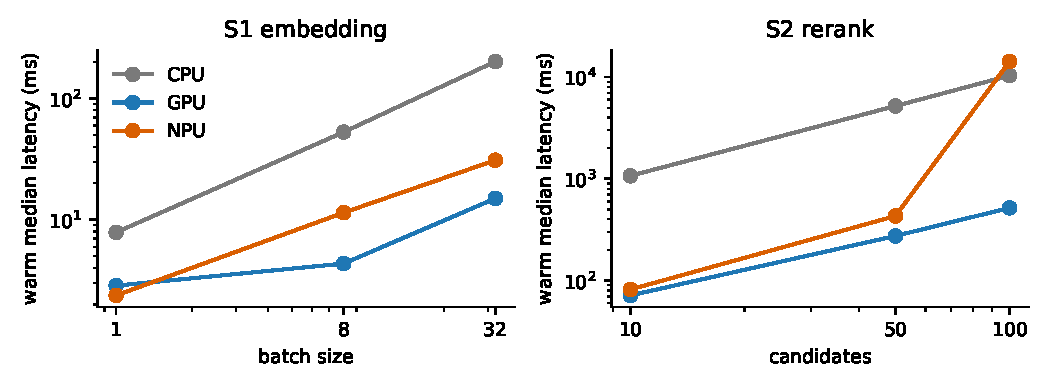
\includegraphics[width=0.72\linewidth]{figs/fig_stage.pdf}
\caption{Warm median latency of S1 and S2 (log--log), first Phase 1 sweep; Table~\ref{tab:s12} uses the Phase 1b rerun, which agrees within a few percent except S1 on the iGPU at batch 1. S2 on the NPU needs 4 min (50 candidates) and 21 min (100 candidates) to compile.}\label{fig:stage}
\end{figure}

\begin{table}[!htb]\centering\small
\caption{S1 and S2 warm median latency (ms), Phase 1b run, 10 repetitions.}\label{tab:s12}
\begin{tabular}{lrrrrrrr}\toprule
 & \multicolumn{3}{c}{S1, batch} & \multicolumn{4}{c}{S2, candidates}\\
\cmidrule(lr){2-4}\cmidrule(lr){5-8}
 & 1 & 8 & 32 & 10 & 20 & 50 & 100\\\midrule
CPU & 7.8 & 52.8 & 202 & 1076 & 2092 & 5180 & 10319\\
iGPU & 1.4 & 4.2 & 15.1 & 71 & 129 & 276 & 522\\
NPU & 2.4 & 9.0 & 27.9 & 84 & 173 & 434 & 14200\\\bottomrule
\end{tabular}
\end{table}

\textbf{S1.} All devices take under 10\,ms at batch 1, where the iGPU and NPU are close (iGPU 1.4--2.9\,ms depending on the run, NPU 2.4\,ms) and fixed overhead dominates. The iGPU scales much better (15\,ms at batch 32 versus 28--31\,ms on the NPU), and the CPU scales worst (202\,ms). \textbf{S2.} The iGPU is the best choice from 10 candidates up. The NPU matches it only at 10 candidates, is 1.6$\times$ slower at 50, and collapses at 100 (14\,s).

\begin{figure}[!htb]\centering
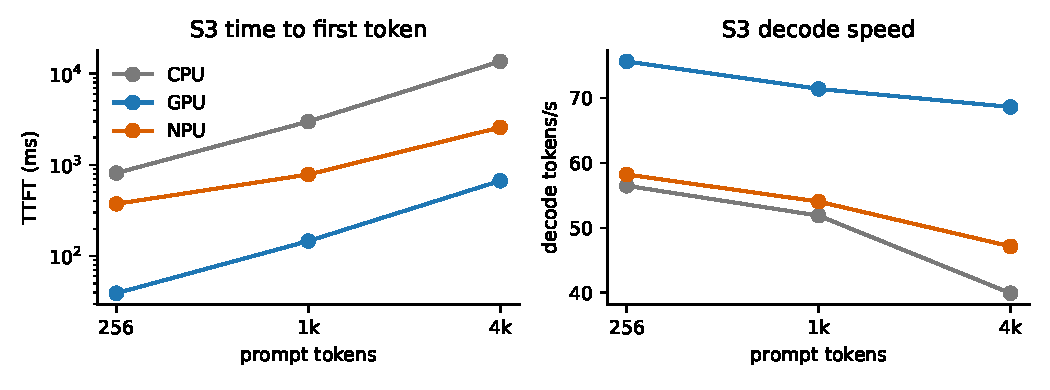
\includegraphics[width=0.72\linewidth]{figs/fig_s3.pdf}
\caption{S3 on synthetic prompts built from corpus text (128 output tokens, fresh prompt per repetition; Oct 27 fresh-prompt sweep, the text quotes the Phase 1b rerun, within 3\%). The NPU was compiled for \texttt{MAX\_PROMPT\_LEN}=4224.}\label{fig:s3}
\end{figure}

\textbf{S3.} Prefill is the large difference (Fig.~\ref{fig:s3}): at 1k tokens TTFT is 146\,ms on the iGPU, 771\,ms on the NPU and 2932\,ms on the CPU. Decode speed is 69--75 tokens/s on the iGPU, 47--58 on the NPU and 40--56 on the CPU; decode is memory-bandwidth bound, so the gap is much smaller than in prefill. On the iGPU, output length does not change TTFT or time per output token (TPOT 13.3--14.6\,ms), so total time is linear in output tokens. The NPU's TTFT depends on the compiled prompt limit rather than the real prompt: a 256-token prompt takes 99.6\,ms with \texttt{MAX\_PROMPT\_LEN}=384 but 366\,ms with 4224, and larger limits also use more device memory (Table~\ref{tab:cost}).

\begin{table}[!htb]\centering\small
\caption{Cost beyond latency (Phase 1b). Load time is the cold start with caches bypassed; memory is added by loading the model.}\label{tab:cost}
\begin{tabular}{llrrp{4.2cm}}\toprule
Stage & Device & Load (s) cached / cold & Memory (MB) & Notes\\\midrule
S1 (b=1) & iGPU & 0.44 / 0.98 & 130 & \\
S1 (b=1) & NPU & 0.07 / 0.98 & 67 & \\
S2 (20 cand.) & iGPU & 3.1 / 3.8 & 596--818 & \\
S2 (20 cand.) & NPU & 0.12 / 68 & 726 & 242\,s for 50 cand.\\
S3 & iGPU & 1.6 / 3.0 & 1002 & \\
S3 & NPU & 4.9 / 10.7 & 1355 / 1893 / 2030 & for \texttt{MAX\_PROMPT\_LEN} 384 / 1152 / 4224; cached load 2.0 / 4.9 / 6.2\,s\\
S3 & CPU & 0.7 / 0.7 & (host RAM) & \\\bottomrule
\end{tabular}
\end{table}

An uncached NPU compile also needs 1.7--3.2\,GB of host RAM, and a whole end-to-end process uses 1.7--2.4\,GB of RSS, so memory is not a constraint on this machine, but the NPU LLM's footprint grows with its static prompt shape.

\textbf{Data movement.} Because the devices share DRAM, ``transfer'' is a host-side copy, not a bus crossing, and the payload between stages is small (per query: 1.5\,KB query vector, 14.6\,KB of candidate text, 2.4\,KB prompt). Input transfer is also cheap: the iGPU reranker's input copy is 3--13\,ms and the NPU's is under 0.4\,ms. Reranker tokenization (8--35\,ms, 10--15\% of iGPU S2) is a larger host-side cost; S3 tokenization and detokenization take under 2\,ms. The first inference after loading is also slower: 8--12\,ms extra for S1 on the iGPU, and up to 2$\times$ the warm latency for S2 on the NPU (199 versus 84\,ms at 10 candidates).

\section{End-to-end results}
\begin{table}[!htb]\centering\small
\caption{All 27 mappings were measured; S1 is shown on the iGPU (S1 on CPU or NPU changes latency by at most 22\,ms in every row). Sequential, 100 dev questions per round. $n$ = questions measured.}\label{tab:e2e}
\begin{tabular}{llrrrr}\toprule
S2 & S3 & Median (ms) & p90 (ms) & q/s & $n$\\\midrule
iGPU & iGPU & \textbf{437} & 621 & \textbf{2.23} & 300\\
NPU & iGPU & 573 & 757 & 1.73 & 300\\
CPU & iGPU & 2437 & 2624 & 0.41 & 300\\
iGPU & NPU & 843 & 1093 & 1.19 & 200\\
NPU & NPU & 825 & 1103 & 1.19 & 100\\
CPU & NPU & 2831 & 3091 & 0.35 & 100\\
iGPU & CPU & 1866 & 2445 & 0.52 & 100\\
NPU & CPU & 1991 & 2423 & 0.51 & 100\\
CPU & CPU & 3845 & 4384 & 0.26 & 100\\\bottomrule
\end{tabular}
\end{table}

With S3 on the iGPU, a query takes 437\,ms: S1 2\,ms, search 4\,ms, S2 118\,ms, S3 316\,ms (TTFT 81\,ms). Putting S3 on the NPU doubles the latency, and on the CPU it multiplies it by 4. S2 on the NPU does not help sequentially (231\,ms versus 118\,ms) because the NPU reranker is slower than the iGPU's; with overlapped execution, where S2 of the next query runs while S3 decodes, S2 on the NPU reaches 2.45--2.50 queries/s versus 2.38 for all-iGPU, a gain of about 5\%. All-iGPU gains only 7\% from overlap (2.23 to 2.38) because both stages share one device, whereas S2 on the NPU gains 44\% over its own sequential run (1.74 to 2.50); S3 on the iGPU then slows from 316 to about 385\,ms (Sec.~\ref{sec:cont}). Placement also affects output: the NPU reranker reorders candidates (recall@3 0.87 $\rightarrow$ 0.82--0.83), while S2 on the CPU and iGPU rank identically. Real RAG prompts are shorter than the 1k/4k sweep points: top-1/3/8 passages give 213/555/1379 tokens (max 1888), and top-8 takes 764\,ms end to end on the iGPU (TTFT 247\,ms) and 1342\,ms with S3 on the NPU.

\subsection{Load}
\begin{figure}[!htb]\centering
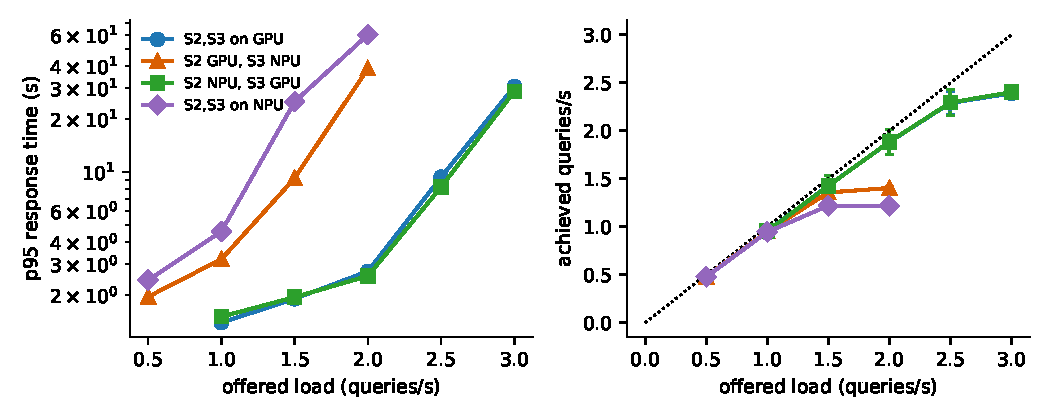
\includegraphics[width=0.72\linewidth]{figs/fig_load.pdf}
\caption{Open-loop Poisson arrivals (3 rounds, at least 150 queries per point; error bars: std over rounds). Response time includes queueing.}\label{fig:load}
\end{figure}

Every mapping behaves like a queue with a hard capacity (Fig.~\ref{fig:load}): below it, response time is close to the service time; above it, waiting grows without bound (p50 of 42\,s at 2.0 q/s for S2 and S3 on the NPU). Capacity is 2.4 q/s for S3 on the iGPU and 1.2--1.4 for S3 on the NPU. Between the two S3-on-iGPU mappings the evidence is mixed: in closed-loop runs S2 on the NPU gives 2.45--2.49 q/s versus 2.38 (+4\%), but under Poisson arrivals the two have the same capacity within noise (2.39 vs 2.40, std 0.12--0.14 q/s), the same p50 at 2.0 q/s, and a 12\% lower p95 at 2.5 q/s for the NPU variant. At 1 q/s all-iGPU has the lower median (0.61 versus 0.73\,s). Hence any benefit of an NPU reranker appears only near saturation and is small.

\subsection{Why concurrent devices interfere}\label{sec:cont}
Running S3 decode next to a reranker on another device (Table~\ref{tab:cont}) causes the same slowdown from a thread or a separate process, and none from a tokenize-only thread, so the cause is not the Python GIL but shared memory bandwidth: iGPU TPOT rises 58\% next to an NPU reranker and NPU TPOT 70\% next to an iGPU reranker, while a CPU reranker costs only 8\%. This is why overlapped pipelines gain much less than the sum of their parts.

\begin{table}[!htb]\centering\small
\caption{S3 decode (1k-token prompt, 128 output tokens) with an S2 reranker running elsewhere.}\label{tab:cont}
\begin{tabular}{lllrr}\toprule
S3 device & Aggressor & Mode & TTFT (ms) & TPOT (ms)\\\midrule
iGPU & none & -- & 148 & 14.0\\
iGPU & rerank on NPU & thread / process & 191 & 22.1\\
iGPU & tokenize only & thread & 157 & 14.2\\
iGPU & rerank on CPU & process & 162 & 15.2\\
NPU & none & -- & 769 & 18.6\\
NPU & rerank on iGPU & process & 1052 & 31.5\\\bottomrule
\end{tabular}
\end{table}

\section{Device preference}
\begin{table}[!htb]\centering\small
\caption{Which device under which condition (Phase 1 conclusion).}\label{tab:prefer}
\begin{tabular}{p{0.12\linewidth}p{0.3\linewidth}p{0.46\linewidth}}\toprule
Stage & Preferred device & Conditions and exceptions\\\midrule
S1 & iGPU, but any device works & Under 10\,ms per query everywhere; avoid the CPU for batches of 8 or more.\\
S2 & iGPU alone; NPU only when overlapping S3 & NPU only up to 50 candidates with a precompiled shape, and it costs about 4 points of recall@3; never the CPU.\\
S3 & iGPU & NPU is about 1.9$\times$ slower end to end, with TTFT tied to its compiled maximum prompt; CPU only as a fallback.\\
Pipeline & All-iGPU; S2 on the NPU may help only near saturation & Same Poisson capacity ($\approx$2.4\,q/s) within noise; S2 on the NPU gives +4\% closed-loop throughput and 12\% lower p95 at 2.5\,q/s; iGPU+NPU overlap costs up to +58\% S3 TPOT.\\\bottomrule
\end{tabular}
\end{table}

Table~\ref{tab:prefer} summarizes the profiles; they are the inputs to the Phase 2 placement policy.

\section{Limitations}
\begin{itemize}\setlength\itemsep{0pt}
\item \textbf{Two NPU models in one process.} An NPU LLM together with any other NPU model in one process fails at first inference (\texttt{zeMemAllocHost}, null handle), although the same configuration ran on Oct 27. For those mappings the LLM runs in its own process, which adds 0.4--0.6\,ms per call and no measurable end-to-end overhead (842 vs 845\,ms in a control).
\item \textbf{Noise and sample size.} The machine is shared (load average 1--8). Only the main 9 S3-on-iGPU mappings have three rounds; the others have one or two. Quality comparisons use 100 questions with no confidence intervals. The S3 sweep on CPU and NPU covers only 128 output tokens, and its prompts are synthetic.
\item \textbf{Scope.} The corpus is small (25,880 passages), so search is negligible; with a much larger index it would matter. Energy was not measured because power counters need root access, so our comparison is performance only.
\end{itemize}

\appendix
\section{Timeline and milestones}
\begin{table}[h]\centering\small
\begin{tabular}{p{0.16\linewidth}p{0.62\linewidth}l}\toprule
Date & Milestone & Status\\\midrule
Oct 27 & Repository, models (FP16 encoders, INT4-sym LLM), corpus and passage index; device support check; stage sweeps and 9 S1$\times$S2 mappings; S3 sweep rerun with fresh prompts & done\\
Oct 28 & Instrumentation for placement, memory, transfer and true cold start; concurrency (closed-loop, Poisson) and contention runs & done\\
Nov 1 & Remaining mappings (all 27), load sweep, top-$N$ prompt sizes & done\\
Nov 2 & NPU two-model workaround (S3 in its own process) and remeasurement & done\\
Nov 4 & \textbf{Phase 1 report} & this report\\\midrule
Nov 5--13 & Placement policy (lookup table / performance model from the Phase 1 profiles); policy decision overhead & planned\\
Nov 14--20 & Baselines (fixed mappings, best static mapping on dev); evaluation on held-out HotpotQA and a mixed short/long prompt workload & planned\\
Nov 21--27 & Policy under concurrent load, including switching (model load) and transfer cost; S2 length-bucketed batches and per-class NPU \texttt{MAX\_PROMPT\_LEN} & planned\\
Nov 28--Dec 3 & Qwen2.5-3B sensitivity check; confidence intervals for quality differences & planned\\
Dec 4--10 & \textbf{Final report} (due Dec 10) & planned\\\bottomrule
\end{tabular}
\end{table}
\end{document}
